 \chapter{Getting Started}
%TODO: Incomplet, ``l'exercice'' propos� en fin de chapitre est ridiculement restreint pour l'instant.

 There are several usage scenario for the \ma. We present here the interactive
 use of the tool. The goal of this chapter is to get you familiar with the \ma's
 interface in half an hour. We assume you have already installed the tool .

 \section{Launching the \ma}
 First ensure that you have copied your personal license file to the
 \texttt{license} folder (cf. \S \ref{AddingLicenseYourFile}). Launch the
 \ma with \texttt{Start -> Programs -> Midlet Analyser -> Start}
 on Windows, or by typing \texttt{matos} in a Linux shell. The
 window shown on figure \ref{figGUIMainWin} appears. 
 
\ifthenelse{\equal{\Gallery}{true}}{ 
 \begin{figure}[h]
 \begin{center}
 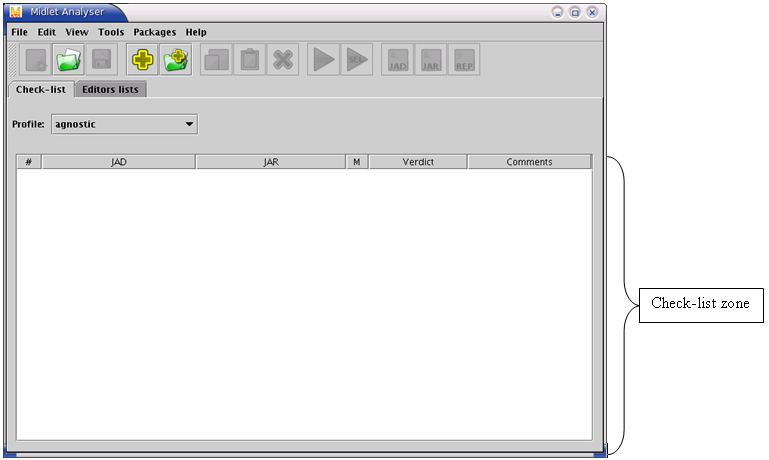
\includegraphics[width=14cm]{figures/GUI-main-Gallery}
 \end{center}
 \caption{Graphical user interface, main window}
 \label{figGUIMainWin}
 \end{figure}
}{
 \begin{figure}[h]
 \begin{center}
 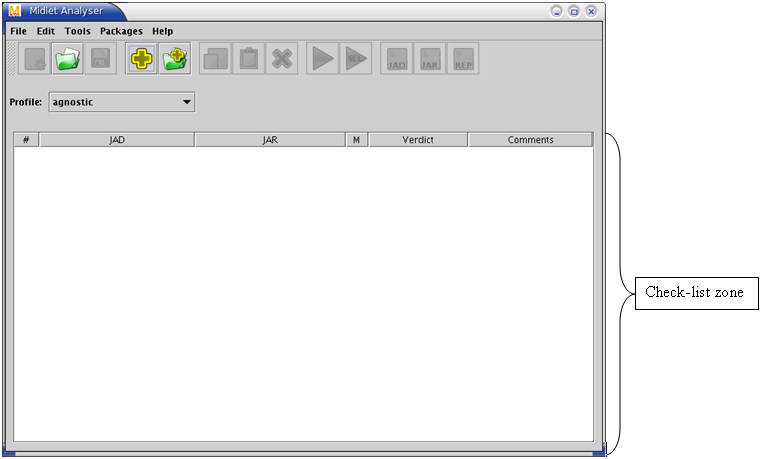
\includegraphics[width=14cm]{figures/figures/GUI-main-OP}
 \end{center}
 \caption{Graphical user interface, main window}
 \label{figGUIMainWin}
 \end{figure}
}

 \subsection*{The check-list zone}
 The main part of the interface is called the \emph{check-list} zone. It is a table
 representing what analyses are going to be performed when you start
 the process. An analysis, represented by a single row in the
 table, is also called a \emph{check-step}. It is one step among all the steps
 of the sequence.
 \subsection*{Keep music in mind!} 
 The concept of check-list is very similar to the concept of \textbf{play-list}
 in an audio player such as Windows Media Player\texttrademark. In an
 audio player, you define a list of songs you want the tool to
 play back: you can add songs from your hard disk to the play-list (one
 by one or a whole directory), remove some from the list, maybe change
 some properties (MP3 tags?) of the songs, then finally PLAY the whole
 list. You can even save the play-list you've defined if you like it,
 so you can replay it exactly the same way tomorrow.  

 In the \ma, you manage check-lists instead of play-lists. You define
 a list of analyses you want the tool to execute. You can add an analysis
 for a MIDlet file located on your hard disk or on the Web, add an
 analysis for each MIDlet file of a directory, remove analyses from the
 check-list, change some properties of analyses, then ``PLAY'' the global
 analysis process. In the \ma too you can save and load back your
 check-lists.


 \section{Checking a MIDlet suite}

Let's analyse a single JAR file. In chapter \ref{BasicUsage}, you will find how to analyse a series of
files, and more.

 \begin{figure}[h]
 \begin{center}
 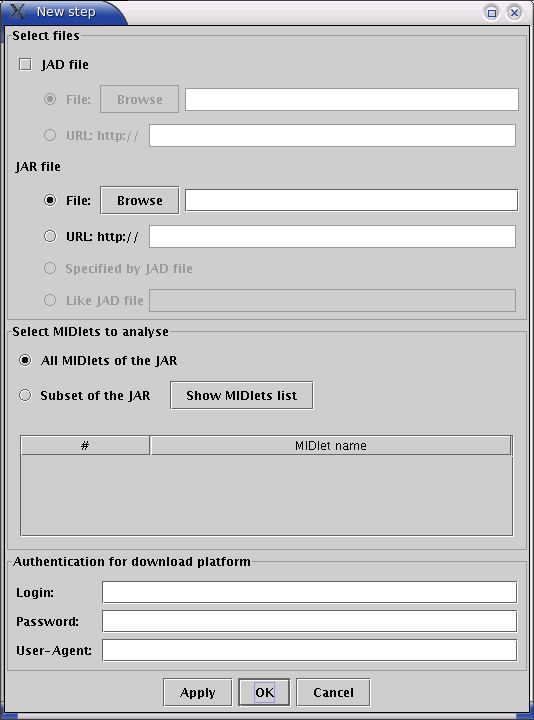
\includegraphics[width=10cm]{figures/GUI-new-step-dialog}
 \end{center}
 \caption{Adding a new check-step (one single MIDlet suite)}
 \label{figAddingMIDletSuite}
 \end{figure} 

 \begin{figure}[h]
 \begin{center}
 
\includegraphics[width=1.2cm]{figures/buttonAnalyseSelection}
 \end{center}
 \caption{Button to launch analysis of selected step}
 \label{figButAnalyse}
 \end{figure}

 \begin{figure}[h]
 \begin{center}
 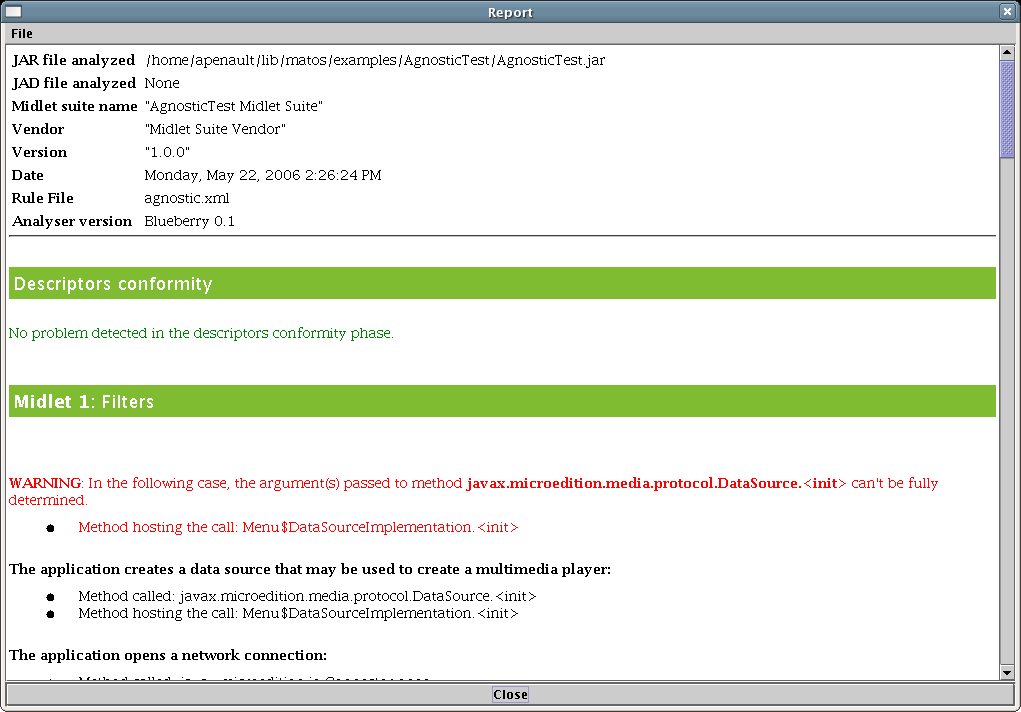
\includegraphics[width=15cm]{figures/reportAgnosticTest}
 \end{center}
 \caption{An example JAR analysis report}
 \label{figExampleReport}
 \end{figure} 
    
 \begin{enumerate}
 \item Select \texttt{File -> Add File to analyse -> Add MIDlet suite...}.
 \item The dialog shown on figure \ref{figAddingMIDletSuite} appears. 
 Since you only want to select a JAR file, ensure the \texttt{JAD file}
 option is unchecked. To specify the JAR you want, select
 \texttt{File:} in the \texttt{JAR file} zone and click
 \texttt{Browse}. Select a JAR file somewhere on your hard disk; you
 may find one in the \texttt{examples} folder of the installation
 directory, such as \texttt{AgnosticTest.jar}.
 \item Make sure the set of MIDlets to analyse is set to \texttt{All MIDlets of
 the JAR}.
 \item Click \texttt{OK}. As you can see, the check-list now contains
   one step (\#1), representing the analysis you've just
   specified. On the main window, select \texttt{agnostic} for the profile.
 \item{Click on the button shown on figure \ref{figButAnalyse} to
 analyse the selected step.} 
 \item A dialog appears, you must indicate the folder for the analysis results.
 \item When the analysis process is done, click on \texttt{Close} button. A
 window opens to show you the report. For the \texttt{AgnosticTest.jar} example
   the report window should look as shown on figure
   \ref{figExampleReport}.
 \end{enumerate}

All analysis reports are divided into three parts:
\begin{itemize}
\item The fist part until the horizontal separator identifies the MIDlet analysed and 
  summarizes the main characteristics of the analysis:
  \begin{itemize}
  \item the name of the jar file analysed
  \item the name of the jad file if one was present
  \item the name of the MIDlet suite, as registered in the manifest or in the JAD file
  \item the MIDlet vendor and the version of the suite
  \item the date of the analysis
  \item the analysis profile (rule file) used
  \item the version of the \ma
  \end{itemize}
\item the next section summarizes the error found in the
  JAD file or in the manifest such as mandatory attributes not defined
  or attributes repeated with different values.
\item the last part consists of one diagnostic section per MIDlet
  analysed. The meaning of the verdicts depends on the analysis profile
  chosen and is out of the scope of this manual. 
  
  As a \emph{convention}, PASS verdicts are written in green and FAIL verdicts are written in
  red. Warnings are written in orange and correspond to points the
  evaluator should check manually. Informative text without a priori judgement
  is written in black.
\end{itemize}

\section{Analyzing several midlets}
\subsection{Building a checklist}
\begin{figure}[h]
	\begin{center}
    	\scalebox{0.8}{
\includegraphics{figures/buttonAnalyseAll}}
   	\end{center}
   	\caption{Button to launch analysis of all steps in the current check-list}
   	\label{butAnalyseAll}
\end{figure}

\begin{itemize}
  \item Select \texttt{File -> Add directory}
  \item Select a directory with several midlets. For example
  \texttt{\${LIB}/examples/test/HttpConnection}. Three midlets should appear.
  \item Add another midlet with \texttt{File -> Add file to analyze -> Add
  MIDlet suite} and select a midlet on your hard disk.
  \item Now you have five midlets selected. You can remove one by selecting it
  and pressing the right mouse button to open the contextual menu. Then press
  remove (It removes the midlet from your check-list, not from your computer).
  \item Press the button shown on figure \ref{butAnalyseAll}.
\end{itemize}

\subsection{Saving and recovering a check-list}
\begin{itemize}
  \item Select \texttt{File -> Save as}
  \item Provide a file name for your check-list and press ``Save check-list''
  \item Now you can quit the tool and launch it again. Select \texttt{File ->
  Open} 
  \item type-in the name of your saved check-list. The elements to analyze are
   back.
\end{itemize}
\ifthenelse{\equal{\Gallery}{true}}{
\subsection{Registering and analysing an editor's list}
\textbf{This section is only relevant in the context of the Gallery portal.}
% \vspace{0.5cm}
% \begin{tabbing}
%  \hspace{0.4cm} \= 1. \hspace{1pt} \= Select \texttt{File -> Register} an editor's list.\\\\
%  \> 2. \> Select an editor's list (an Excel file) somewhere on your hard disk. A
%  row appears on the table in the \\ \> \> \texttt{Editors lists} tab.\\\\
%  \> 3. \> Select the added row and click on the \texttt{Add to check-list}
%  button. All JAR and JAD files described in \\ \> \> the editor's list are added
%  in the current check-list.\\\\
%  \> 4. \> To analyse all steps of the current check-list, click on the button
%  shown on figure \ref{butAnalyseAll}.
% \end{tabbing}
\begin{itemize}
 \item Select \texttt{File -> Register an editor's list\ldots}
 \item Select an editor's list (an Excel file) somewhere on your hard disk. A
 row appears on the table in the \texttt{Editors lists} tab.
 \item Select the added row and click on the \texttt{Add to check-list}
 button. All JAR and JAD files described in the editor's list are added
 in the current check-list.
 \item To analyse all steps of the current check-list, click on the button
 shown on figure \ref{butAnalyseAll}.
\end{itemize}
}{}


%% POSTPONED
%% \paragraph{Exercise B}
%%  %TODO
%%  [scenario2 : add a JAD [HTTP address], analyse all, popup/view report,
%%  close it.]

%%  \paragraph{Exercise C}
%%  %TODO
%%  [scenario3 : add directory, remove les 2 doublons, force a profile for
%%  all, save as, analyse all, remove all, open the saved one.]

\section{The Command Line Mode} \label{CmdLineMode}
The \ma can be used to some extent in command line mode. The main
command is called \texttt{matos}. The general syntax is:
\begin{alltt}
matos \emph{[options] [parameter]} 
\end{alltt}

When only one pararmeter is present and it is a JAR or JAD file, the tool
is launched in interactive mode. 
The GUI will open and get prepared for the analysis of the specified file (it
is added to the check-list zone). Refer to  \ref{IdentTargetFiles} to see what
happens if the parameter is a JAD file.

When at least one option is specified, the GUI won't open, and the
tool will execute fully as a batch shell command.

\subsection{Options}

\newcommand{\OptArg}[2]{\textsf{#1~\textit{#2}}}
\newcommand{\Opt}[1]{\textsf{#1}\xspace}
\newcommand{\File}[1]{\textit{#1}\xspace}
\begin{description}
%\item[\OptArg{-t }{transfile}]\setlength{\itemsep}{0cm}

\item[\OptArg{-jar }{jar-file-name}] Force the target JAR file. When
  this option is used while a JAD file is specified (using the parameter or \texttt{-jad}), the JAR URL
  specified into the JAD file is ignored. This option may also be used
  if the wanted JAR file does not carry the standard \texttt{.jar}
  extension.  This option is ignored when \texttt{-c} is used.

\item[\OptArg{-jad }{jad-file-name}] Force the target JAD file. May
  also be used if the wanted JAD file does not carry the standard \texttt{.jad}
  extension. This option is ignored when \texttt{-c} is used.
\item[\OptArg{-apk }{apk-file-name}] Force the target Android APK file. May
  also be used if the wanted APK file does not carry the standard \texttt{.apk}
  extension. This option is ignored when \texttt{-c} is used.
\item[\OptArg{-d }{profile-name}] Use the specified security profile. 
Valid profile names are those of XML files present in the 
\File{\emph{install-Matos}/lib/definitions} directory, without the
extension. This option is ignored when \texttt{-c} is used.

\item[\OptArg{-o }{output-file-name}] Output results to the specified
  output file. By default the output goes to a file called
  \texttt{output.html}. If \texttt{-c} is used, \texttt{-o} is assumed to be
  the output \emph{directory} where to store all results of the
  check-list execution. %TODO: c'est quoi le dir cr�� par d�faut ?

\item[\Opt{-pdf}] Export the output results in PDF format, the generated PDF
file as the same name and the same location as the file specified in the \texttt{-o}
option. If \texttt{-pdf} is used, the use of \texttt{-o} option is mandatory.

\item[\OptArg{-m }{midlet-name}] Among all the MIDlets contained in
  the target MIDlet suite, run the analysis for the specified MIDlet
  only. This option allows to specify explicitly what MIDlets should
  be analysed. By default, all MIDlets of the target JAR are
  analysed. To target explicitly more than one MIDlet, use multiple
  instances of this option. The MIDlet name must be a fully qualified
  MIDlet Identifier (packages names included, eg. \texttt{pack1.pack2.MyFirstMidlet}).
  This option is ignored when \texttt{-c} is used.

\item[\OptArg{-c }{check-list-file-name}] Run in check-list mode (also called ``campaign''). 
Execute the sequence of analyses specified in the check-list file
provided. Such files are \texttt{.mcl} files as those saved from the GUI. The
\texttt{-o} option here can be used to specify the output directory where to
produce all results files.  The following options are ignored when \texttt{-c}
is used: \texttt{-d},\texttt{-m},\texttt{-jar},\texttt{-jad},\texttt{-all}.

\item[\OptArg{-all }{dir-name}] Run the analysis on all application files found
  present in the specified directory. For midlets, all JAD files are taken first,
  for which the \ma uses the \texttt{MIDlet-Jar-URL} attribute to locate the
  corresponding JAR file. These files are analysed, then so are all JAR
  files of the specified directory that were not treated already
  (those that are not pointed to by JAD file). The \texttt{-all}
  option is ignored when \texttt{-c} is used.

\item[\OptArg{-tmp }{dir-name}] Ask the tool to use the specified directory as a
  temporary directory. Warning: the \ma may take the freedom to
  destroy this directory when not needed anymore. By default, the
  system's main temporary directory is used, stored in the \texttt{TEMP} environment variable.

\item[\OptArg{-css }{file-name}] Ask the tool to use the specified
  style sheet for the final presentation of the HTML output file. By
  default no presentation is applied. Please note that a ready-to-use style
  sheet called \texttt{style.css} is provided in the installation
  directory. The user is free to use that file with the \texttt{-css}
  option.
  
\item[\OptArg{-log }{file-name}] Put logs generated by the \ma during its
execution in the specified file. By default logs goes to a file called
  \texttt{log.txt} in the \File{\emph{install-Matos}/lib/} directory.

\item[\Opt{-apache}] Adapt the HTML output when the \ma is invoked
  through a web server. In particular, only the body of the document
  is generated, rather than a complete HTML document with enclosing
  \texttt{<html>} tags. In addition, the actual path of the analysed
  files is not shown in the header of the results report.
\item[\OptArg{-tmp }{dir-name}] change the temporary folder used to \verb!dir-name!.
\item[\Opt{-xml}] Output the result in XML format (\texttt{-o} must be used).  

\item[\Opt{-h}] Online help.

\end{description}

\subsection{Identification of target files}\label{IdentTargetFiles}
The files to be analysed are specified to the \ma by indicating a
path to them. The path is either a path which is relative to the
working directory or a classical HTTP URL starting with \texttt{http://}.

If the only file specified is a JAD file, the corresponding JAR
will be searched at the location specified by the 
\texttt{MIDlet-Jar-URL} attribute, in the JAD. If that attribute is
not a well-formed HTTP URL, \emph{while} the specified JAD path is
an HTTP URL, then the JAR file will be searched at the same location
as the JAD. For example, if the option
\texttt{-jad "http://www.supermidlets.com/fun/pingpong.jad"} is
specified, while the JAD contains the attribute
\texttt{MIDlet-Jar-URL: pingpong.jar}, then the tool will assume the JAR
file address is actually
\texttt{http://www.supermidlets.com/fun/pingpong.jar}.

This remark applies however the target file(s) was specified (main argument of the textual command, -jad or -jar flags, or
the \texttt{jar} or \texttt{jad} attributes in the check-list file, when
run in check-list mode).

\subsection{Examples}

\begin{itemize}
\item{\texttt{matos}}\\ 
Starts the \ma in interactive mode. The GUI is opened, with no focus
on a particular target file.
\item{\texttt{matos Pacman.jar}}\\
Starts the \ma in interactive mode. The GUI is opened in MIDP mode, with focus
on the Pacman.jar file. That file is added to the current check-list.
\item{\texttt{matos Pacman.apk}}\\
Starts the \ma in interactive mode. The GUI is opened in Android mode, with
focus on the Pacman.apk file which is an Android application. 
That file is added to the current check-list.
\item{\texttt{matos -jar Pacman.jar}}\\
Launches directly the analysis of Pacman.jar. The GUI is not opened. Since nothing more is
specified, the analysis profile used will be the one set as default in
the tool configuration. 
\item{\texttt{matos -jar Pacman.jar -o PacmanResults.html -d
    agnostic}}\\
Launches directly the analysis of Pacman.jar, using the Agnostic
security profile. The GUI is not opened. Reporting is produced in the PacmanResults.html
file.
\item{\texttt{matos -jad Pacman.jad}}\\
Only the JAD is provided here: the tool will search for its associated
JAR at the location indicated by the \texttt{MIDlet-Jar-URL} attribute
of the JAD.
\end{itemize}

%%% Local Variables: 
%%% mode: latex
%%% TeX-master: "Users-manual"
%%% End: 
